% !TEX program = pdflatex
% 固体物理第十二次作业
\documentclass[UTF8,10pt,a4paper]{article}
\usepackage{ctex}
% \catcode`\。=\active
% \newcommand{。}{.}
\newcommand{\CourseName}{固体物理}
\newcommand{\CourseCode}{PHYS1502}
\newcommand{\Semester}{2019-2020学年第二学期}
\newcommand{\ProjectName}{第十二次作业}
\newcommand{\DueTimeType}{截止时间}
\newcommand{\DueTime}{2020. 5. 29(周五)17:00}
\newcommand{\StudentName}{陈稼霖}
\newcommand{\StudentID}{45875852}
\usepackage[vmargin=1in,hmargin=.5in]{geometry}
\usepackage{fancyhdr}
\usepackage{lastpage}
\usepackage{calc}
\pagestyle{fancy}
\fancyhf{}
\fancyhead[L]{\CourseName}
\fancyhead[C]{\ProjectName}
\fancyhead[R]{\StudentName}
\fancyfoot[R]{\thepage\ / \pageref{LastPage}}
\setlength\headheight{12pt}
\fancypagestyle{FirstPageStyle}{
    \fancyhf{}
    \fancyhead[L]{\CourseName\\
        \CourseCode\\
        \Semester}
    \fancyhead[C]{{\Huge\bfseries\ProjectName}\\
        \DueTimeType\ : \DueTime}
    \fancyhead[R]{姓名 : \makebox[\widthof{\StudentID}][s]{\StudentName}\\
        学号 : \StudentID\\
        成绩 : \underline{\makebox[\widthof{\StudentID}]{}}}
    \fancyfoot[R]{\thepage\ / \pageref{LastPage}}
    \setlength\headheight{36pt}
}
\usepackage{amsmath,amssymb,amsthm,bm}
\allowdisplaybreaks[4]
\newtheoremstyle{Problem}
{}
{}
{}
{}
{\bfseries}
{.}
{ }
{第\thmnumber{ #2}\thmname{ #1}\thmnote{ (#3)} 得分: \underline{\qquad\qquad}}
\theoremstyle{Problem}
\newtheorem{prob}{题}
\newtheoremstyle{Solution}
{}
{}
{}
{}
{\bfseries}
{:}
{ }
{\thmname{#1}}
\makeatletter
\def\@endtheorem{\qed\endtrivlist\@endpefalse}
\makeatother
\theoremstyle{Solution}
\newtheorem*{sol}{解}
\providecommand{\abs}[1]{\left\lvert#1\right\rvert}
\usepackage{graphicx}
\begin{document}
\thispagestyle{FirstPageStyle}
\begin{prob}[(17.1) Holes]
    \begin{enumerate}
        \item[(a)] In semiconductor physics, what is meant by a hole and why is it useful?
        \item[(b)] An electron near the top of the valence band in a semiconductor has energy
        \[
            E=-10^{-37}\abs{\bm{k}}^2
        \]
        where $E$ is in Joules and $k$ is in m$^{-1}$. An electron is removed from a state $\bm{k}=2\times 10^8\text{m}^{-1}\hat{x}$, where $\hat{x}$ is the unit vector in the $x$-direction. For a hole, calculate (and give the sign of!)
        \begin{enumerate}
            \item[(i)] the effective mass
            \item[(ii)] the energy
            \item[(iii)] the momentum
            \item[(iv)] the velocity
        \end{enumerate}
        \begin{itemize}
            \item[$\triangleright$] If there is a density $\rho=10^5\text{m}^{-3}$ of such holes all having almost exactly this same momentum, calculate the current density and its sign.
        \end{itemize}
    \end{enumerate}
\end{prob}
\begin{sol}
    \begin{enumerate}
        \item[(a)] \textbf{空穴}:当一个电子被从价带上激发到导带上,它在价带上留下的空位就是空穴.\\
        空穴这一概念很有用,因为,未填满的价带上的大量电子的复杂流动导致的电流可以用少数空穴作为载流子流动产生的电流等价代替,简化了问题.
        \item[(b)] 产生一个空穴,等价于移除一个电子,所以空穴的能量与电子的能量相反,因移除电子的能量为$E=-10^{-37}\abs{\bm{k}}^2$,故对应空穴的能量为
        \begin{align}
            E_h=-E=+10^{-37}\abs{\bm{k}}^2=+4\times 10^{-21}\text{J}.
        \end{align}
        空穴的有效质量为
        \begin{align}
            m_h^*=\frac{\hbar^2\abs{\bm{k}}^2}{2E_h}=+5.6\times 10^{-32}\text{kg}.
        \end{align}
        量子态对应的速度与该量子态上填充的粒子是电子还是空穴无关,故空穴的速度与电子的速度相同,为
        \begin{align}
            \bm{v}_h=\bm{v}_e=\frac{\nabla_kE}{\hbar}=-\frac{2\times 10^{-37}\bm{k}}{\hbar}=-3.8\times 10^5\text{m}/\text{s}\,\hat{x}.
        \end{align}
        (沿负$x$方向)\\
        空穴的动量为
        \begin{align}
            \bm{p}=m_h^*\bm{v}_h=-2.1\times 10^{-26}\text{kg}\cdot\text{m}/\text{s}\,\hat{x}.
        \end{align}
        (沿负$x$方向)
        \begin{itemize}
            \item[$\triangleright$] 电流密度为
            \begin{align}
                \bm{J}=\rho e\bm{v}=-6.1\times 10^{-9}\text{A}/\text{m}^2\,\hat{x}.
            \end{align}
            (沿负$x$方向)
        \end{itemize}
    \end{enumerate}
\end{sol}

\begin{prob}[(17.3) Law of Mass Action and Doping of Semiconductors]
    \begin{enumerate}
        \item[(a)] Assume that the band-gap energy $E_g$ is much greater than the temperature $k_BT$. Show that in a pure semiconductor at a fixed $T$, the product of the number electrons ($n$) and the product of the number of holes ($p$) depends only on the density of states in the conduction band and the density of states in the valence band (through their effective masses), and on the band-gap energy.
        \begin{itemize}
            \item[$\triangleright$] Derive expression for $n$ for $p$ and for the product $np$. You may need to use the integral $\int_0^{\infty}dx\,x^{1/2}e^{-x}=\sqrt{\pi}/2$.
        \end{itemize}
        \item[(b)] The band gaps of silicon and germanium are $1.1$ eV and $0.75$ eV respectively. You may assume the effective masses for silicon and germanium are isotropic, roughly the same, and are roughly $.5$ of the bare electron mass for both electrons and holes. (Actually the effective masses are not quite the same, and futhermore the effective masses are both rather anisotropic, but we are just making a rough estimate here.)
        \begin{itemize}
            \item[$\triangleright$] Estimate the conduction electron concentration for intrinsic (undoped) silicon at room temperature.
            \item[$\triangleright$] Make a rough estimate of the maximum concentration of ionized impurities that will still allow for this "intrinsic" behavior.
            \item[$\triangleright$] Estimate the conduction electron concentration for germanium at room temperature.
        \end{itemize}
        \item[(c)] The graph in Fig 17.6 shows the relationship between charger-carrier concentration for a certain $n$-doped semiconductor.
        \begin{itemize}
            \item[$\triangleright$] Estimate the band gap for the semiconductor and the concentration of donor ions.
            \item[$\triangleright$] Describe in detail an experimental method by which these data could have been measured, and suggest possible source of experimental error.
        \end{itemize}
    \end{enumerate}
    \begin{figure}[h]
        \centering
        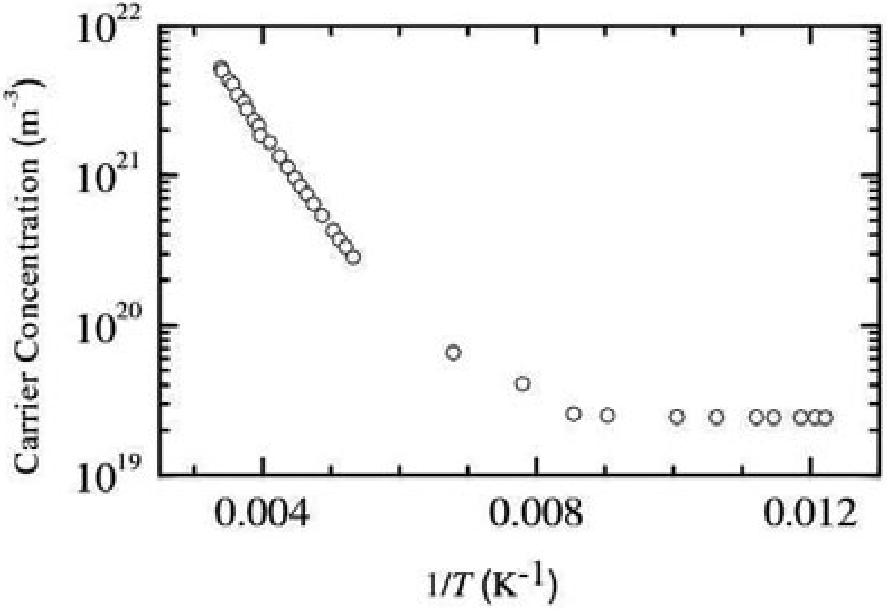
\includegraphics[width=.4\textwidth]{2.png}
        \caption{Fig 17.6 Figure for Exercise 17.2}
    \end{figure}
\end{prob}
\begin{sol}
    \begin{enumerate}
        \item[(a)] 
        \begin{itemize}
            \item[$\triangleright$] 自由电子的态密度为
            \begin{align}
                g(\varepsilon\geq 0)=\frac{(2m)^{3/2}}{2\pi^2\hbar^3}\varepsilon^{1/2}d\varepsilon.
            \end{align}
            除了最低能量为导带最低点$\varepsilon_c$和具有特殊的有效质量$m_e^*$外,导带上的电子与自由电子相当,故其态密度为
            \begin{align}
                g_c(\varepsilon\geq\varepsilon_c)=\frac{(2m_e^*)^{3/2}}{2\pi^2\hbar^3}\sqrt{\varepsilon-\varepsilon_c}.
            \end{align}
            导带上的电子数为
            \begin{align}
                n(T)=\int_{\varepsilon_c}^{\infty}d\varepsilon\,g_c(\varepsilon)n_F(\beta(\varepsilon-\mu)),
            \end{align}
            其中费米填充因子
            \begin{align}
                n_F(\beta(\varepsilon-\mu))=\frac{1}{e^{\beta(\varepsilon-\mu)}+1}.
            \end{align}
            当带隙$E_g$远大于室温$k_BT$,我们有理由假设$\beta(\varepsilon-\mu)\gg 1$,从而费米填充因子
            \begin{align}
                n_F(\beta(\varepsilon-\mu))\approx e^{-\beta(\varepsilon-\mu)}.
            \end{align}
            导带上的电子数为
            \begin{align}
                \nonumber n(T)\approx&\int_{\varepsilon_c}^{\infty}d\varepsilon\,g_c(\varepsilon)e^{-\beta(\varepsilon-\mu)}\\
                \nonumber=&\frac{(2m_e^*)^{3/2}}{2\pi^2\hbar^3}\int_{\varepsilon_c}^{\infty}d\varepsilon\,(\varepsilon-\varepsilon_c)^{1/2}e^{-\beta(\varepsilon-\mu)}\\
                =&\frac{(2m_e^*)^{3/2}}{2\pi^2\hbar^3}e^{\beta(\mu-\varepsilon_c)}\int_{\varepsilon_c}^{\infty}d\varepsilon\,(\varepsilon-\varepsilon_c)^{1/2}e^{-\beta(\varepsilon-\varepsilon_c)}.
            \end{align}
            设$x=\beta(\varepsilon-\varepsilon_c)$,则
            \begin{align}
                \label{nT}
                \nonumber n(T)=&\frac{(2m_e^*)^{3/2}}{2\pi^2\hbar^3}e^{\beta(\mu-\varepsilon_c)}\frac{1}{\beta^{3/2}}\int_0^{\infty}dx\,x^{1/2}e^{-x}\\
                =&\frac{(2m_e^*)^{3/2}}{2\pi^2\hbar^3}e^{\beta(\mu-\varepsilon_c)}\frac{1}{\beta^{3/2}}\frac{\sqrt{\pi}}{2}=\frac{1}{4}\left(\frac{2m_e^*k_BT}{\pi\hbar^2}\right)^{3/2}e^{-\beta(\varepsilon_c-\mu)}.
            \end{align}
            同理价带上的空穴的态密度为
            \begin{align}
                g_v(\varepsilon\leq\varepsilon_d)=\frac{(2m_h^*)^{3/2}}{2\pi^2\hbar^3}\sqrt{\varepsilon_v-\varepsilon}.
            \end{align}
            价带上的空穴数为
            \begin{align}
                p(T)=\int_{-\infty}^{\varepsilon_v}d\varepsilon\,g_v(\varepsilon)[1-n_F(\beta(\varepsilon-\mu))].
            \end{align}
            当带隙$E_g$远大于室温$k_BT$,我们有理由假设$e^{\beta(\varepsilon-\mu)}\ll 1$,从而
            \begin{align}
                1-n_F(\beta(\varepsilon-\mu))=\frac{e^{\beta(\varepsilon-\mu)}}{e^{\beta(\varepsilon-\mu)}+1}\approx e^{\beta(\varepsilon-\mu)}.
            \end{align}
            价带上的空穴数为
            \begin{align}
                \label{pT}
                \nonumber p(T)\approx&\int_{-\infty}^{\varepsilon_v}d\varepsilon\,g_v(\varepsilon)e^{\beta(\varepsilon-\mu)}\\
                \nonumber=&\frac{(2m_p^*)^{3/2}}{2\pi^2\hbar^3}\int_{-\infty}^{\varepsilon_v}d\varepsilon\,(\varepsilon_v-\varepsilon)^{1/2}e^{\beta(\varepsilon-\mu)}\\
                =&\frac{(2m_p^*)^{3/2}}{2\pi^2\hbar^3}e^{\beta(\varepsilon_v-\mu)}\int_{-\infty}^{\varepsilon_v}d\varepsilon\,(\varepsilon_v-\varepsilon)^{1/2}e^{\beta(\varepsilon-\varepsilon_v)}.
            \end{align}
            设$x=\beta(\varepsilon_v-\varepsilon)$,则
            \begin{align}
                \nonumber p(T)=&\frac{(2m_p^*)^{3/2}}{2\pi^2\hbar^3}e^{\beta(\varepsilon_v-\mu)}\frac{1}{\beta^{3/2}}\int_0^{\infty}dx\,x^{1/2}e^{-x}\\
                =&\frac{(2m_p^*)^{3/2}}{2\pi^2\hbar^3}e^{\beta(\varepsilon_v-\mu)}\frac{1}{\beta^{3/2}}\frac{\sqrt{\pi}}{2}=\frac{1}{4}\left(\frac{2m_h^*k_BT}{\pi\hbar^2}\right)^{3/2}e^{-\beta(\mu-\varepsilon_v)}.
            \end{align}
            电子数和空穴数之积为
            \begin{align}
                \label{nTpT}
                \nonumber n(T)p(T)=&\frac{1}{16}\left(\frac{2k_BT}{\pi\hbar^2}\right)^3(m_e^*m_h^*)^{3/2}e^{-\beta(\varepsilon_c-\varepsilon_v)}\\
                =&\frac{1}{2}\left(\frac{k_BT}{\pi\hbar^2}\right)^3(m_e^*m_h^*)^{3/2}e^{-\beta E_g}.
            \end{align}
            这一乘积仅依赖于导带上电子的态密度和价带上空穴的密度(是关于电子/空穴的有效质量的函数)以及带隙.
        \end{itemize}
        \item[(b)]
        \begin{itemize}
            \item[$\triangleright$] 室温($300$K)下,纯硅的导电电子密度为
            \begin{align}
                n(T=300\text{K})=\frac{1}{4}\left(\frac{2(m_e/2)k_BT}{\pi\hbar^2}\right)^{3/2}e^{-\beta E_g/2}=5.20\times 10^{15}\text{m}^{-3}.
            \end{align}
            \item[$\triangleright$] 当掺杂的电子数达到$10^{15}\text{m}^{-3}$的数量级时,就会显著地改变纯硅的原有的导电电子密度.
            \item[$\triangleright$] 室温($300$K)下,纯锗的导电电子密度为
            \begin{align}
                n(T=300\text{K})=\frac{1}{4}\left(\frac{2(m_e/2)k_BT}{\pi\hbar^2}\right)^{3/2}e^{-\beta E_g/2}=4.50\times 10^{15}\text{m}^{-3}.
            \end{align}
        \end{itemize}
        \item[(c)]
        \begin{itemize}
            \item[$\triangleright$] 低温下的载流子数密度即为掺杂离子的数密度,故掺杂离子的数密度为$2\times 10^{19}\text{m}^{-3}$.\\
        在高温下,载流子数密度关于温度大致呈如下关系:
        \begin{gather}
            n\sim e^{-E_g/2k_BT},\\
        \Longrightarrow\lg(n)=-\frac{E_g/2k_BT}{\ln(10)}+\text{constant}.
        \end{gather}
        由图17.6,$n\sim 1/T$曲线在高温段的斜率约为$\frac{d[\lg(n)]}{d(1/T)}\approx\frac{21\lg(5)-20\lg(3)}{0.0053-0.0033}=-4757$(国际单位制,单位暂省去),故可解得带隙为
        \begin{gather}
            -\frac{E_g}{2\ln(10)k_B}=-4757,\\
            \Longrightarrow E_g=3.02\times 10^{-19}\text{J}=1.89\text{eV}.
        \end{gather}
            \item[$\triangleright$] 得到图17.6中数据的实验方法:在不同温度下测量半导体的Hall电流,从而推算出载流子数密度. 可能的误差来源:
            \begin{itemize}
                \item 有时候材料中的载流子并非单纯的电子或者单纯的空穴,而是兼有两者,此时材料的总霍尔电阻率由两种的电阻率叠加而成,如果不在计算载流子密度的过程中注意这一点,就会导致结果出问题. 对此可以做如下简单的计算:\\
                对于单一的载流子$i$,外加的电场和该种载流子贡献的电流密度之间的关系为
                \begin{align}
                    \vec{E}=\rho_i\vec{j}_i,
                \end{align}
                其中电阻率矩阵为
                \begin{align}
                    \rho_i=\left(\begin{matrix}
                        r & BR_i\\
                        BR_i & r
                    \end{matrix}\right)
                \end{align}
                其中霍尔系数
                \begin{align}
                    R_i=\frac{1}{n_iq_i},
                \end{align}
                其中$n_i$为$i$类载流子的数密度,$q_i$为$i$类载流子所带的电荷数.
                当材料中同时存在两种载流子$e$(电子)和$h$(空穴)时,外加电场和总电流间的关系为
                \begin{align}
                    \vec{E}=\rho(\vec{j}_e+\vec{j}_h).
                \end{align}
                可以想见,此时的电阻率矩阵是一个与$n_e$(电子的数密度)和$n_h$(空穴的数密度)相关的比较复杂的形式,从这一矩阵的各个矩阵元从中推算载流子数密度一定要小心.
                \item 对电流、磁场控制和测量时产生的误差.
                \item 霍尔电压的测量时如果测量的不是刚好垂直于电流和磁场方向的,会引入误差.
                \item 电压测量时接触电阻会导致电压测量偏大.
            \end{itemize}
        \end{itemize}
    \end{enumerate}
\end{sol}

\begin{prob}[(17.3) Chemical Potential]
    \begin{enumerate}
        \item[(a)] Show that the chemical potential in an intrinsic semiconductor lies in the middle of the gap at low temperature.
        \item[(b)] Explain how the chemical potential varies with temperature if the semiconductor is doped with (i) donors (ii) acceptors.
        \item[(c)] A direct-gap semiconductor is doped to produce a density of $10^{23}$ electrons/m$^3$. Calculate the hole density at room temperature given that the gap is $1.0$ eV, and the effective mass of carriers in the conduction and valence band are $0.25$ and $0.4$ electron masses respectively. Hint: use the result of Exercise 17.2.a.
    \end{enumerate}
\end{prob}
\begin{sol}
    \begin{enumerate}
        \item[(a)] 定性的解释:化学势的定义是体系增加一个电子所导致平均增加的能量. 对于本征半导体,其中的电子满足费米分布,在低温下,其价带几乎被填满,而导带几乎为全空,电子的布居情况差不多关于$[(\varepsilon_c+\varepsilon_v)/2,\frac{1}{2}]$奇对称(回忆一下那张类似与阶跃函数的图,半导体虽然中间有带隙不能填充电子,但意思是这个意思),增加一个电子,导致能量增加的期望值为$(\varepsilon_c+\varepsilon_v)/2$,故其化学势在带隙的中间.\\
        定量的计算:对于本征半导体,其导带上的电子的数量与价带上的空穴的数量相等:
        \begin{align}
            \frac{n(T)}{p(T)}=1.
        \end{align}
        代入前一题中的式\eqref{nT}和式\eqref{pT},得
        \begin{gather}
            \frac{m_e^{*3/2}e^{-\beta(\varepsilon_c-\mu)}}{m_h^{*3/2}e^{-\beta(\mu-\varepsilon_v)}}=1,\\
            \Longrightarrow\mu=\frac{E_c+E_v}{2}+\frac{3}{4}k_BT\ln\left(\frac{m_h^*}{m_e^*}\right).
        \end{gather}
        在低温下($T\rightarrow 0$),
        \begin{align}
            \mu\approx\frac{\varepsilon_c+\varepsilon_v}{2}.
        \end{align}
        \item[(b)] 对于掺杂的情况,
        \begin{align}
            \frac{n(T)}{p(T)}\neq 1.
        \end{align}
        故
        \begin{gather}
            \frac{m_e^{*3/2}e^{-\beta(\varepsilon_c-\mu)}}{m_h^{*3/2}e^{-\beta(\mu-\varepsilon_v)}}=\frac{n(T)}{p(T)},\\
            \Longrightarrow\mu=\frac{E_c+E_v}{2}+\frac{3}{4}k_BT\ln\left(\frac{m_n^*}{m_e^*}\right)+\frac{1}{2}k_BT\ln\left(\frac{n(T)}{p(T)}\right).
        \end{gather}
        (i) 对于施主掺杂的情况,半导体中电子多于空穴,
        \begin{align}
            \frac{n(T)}{n(P)}>1.
        \end{align}
        这导致在低温下($T\rightarrow 0$),
        \begin{align}
            \mu>\frac{\varepsilon_c+\varepsilon_v}{2}
        \end{align}
        (ii) 对于受主掺杂的情况,半导体中空穴多于电子,
        \begin{align}
            \frac{n(T)}{p(T)}<1.
        \end{align}
        这导致在低温下($T\rightarrow 0$),
        \begin{align}
            \mu<\frac{\varepsilon_c+\varepsilon_v}{2}.
        \end{align}
        \item[(c)] 在掺杂前,室温下($T=300$K),电子数和空穴数之积为
        \begin{align}
            n(T)p(T)=\frac{1}{2}\left(\frac{k_BT}{\pi\hbar^2}\right)^3(0.25m_e0.4m_h)^{3/2}e^{-\beta E_g}=3.26\times 10^{32}\text{m}^{-6}.
        \end{align}
        本征半导体的电子数与空穴数相等,故
        \begin{align}
            n(T)=p(T)=\sqrt{n(T)p(T)}=1.80\times 10^{16}\text{m}^{-3}.
        \end{align}
        掺杂后电子密度远大于这一值,掺杂不影响式\eqref{nTpT}右边的任意一个变量,故电子密度与空穴密度之积不变,故掺杂后空穴密度为
        \begin{align}
            p(T)=\frac{3.26\times 10^{32}\text{m}^{-6}}{10^{23}\text{m}^{-3}}=3.26\times 10^9\text{m}^{-3}.
        \end{align}
    \end{enumerate}
\end{sol}

\begin{prob}[(17.5) Semiconductors]
    Describe experiments to determine the following properties of a semiconductor sample: (i) sign of the majority carrier (ii) carrier concentration (assume that one carrier type is dominant) (iii) band gap (iv) effective mass (v) mobility of the majority carrier.
\end{prob}
\begin{sol}
    \begin{enumerate}
        \item[(i)] Hall效应实验:施加垂直于电流$I$的磁场$B$,由半导体在垂直于电流和磁场方向积累的电荷种类,可以推断出载流子在磁场中受到的洛伦兹力方向,从而确定主要的载流子.
        \item[(ii)] Hall效应实验:施加垂直于电流$I$的磁场$B$,测量出样品厚度$d$和Hall电压$V_H$,利用
        \begin{align}
            R_H=\frac{V_Hd}{IB}
        \end{align}
        计算Hall系数,进而用
        \begin{align}
            R_H=\frac{1}{ne}
        \end{align}
        推算出载流子密度.
        \item[(iii)] 用光学方法(测吸收谱)可以测出带隙.
        \item[(iv)] 回旋共振法测量载流子的有效质量:将半导体置于匀强磁场$\bm{B}$中,则其中的载流子具有共振频率
        \begin{align}
            \omega=\frac{qB}{m^*}.
        \end{align}
        此时输入一个交变电磁场(也就是光),当电磁场的频率与载流子的共振频率达到一致,即产生共振吸收现象,从而可以推算出载流子的有效质量.
        \item[(v)] 电导率和迁移率之间存在如下关系:
        \begin{align}
            \sigma=ne\mu.
        \end{align}
        在已知载流子密度的情况下,只需要测量半导体的电导率即可推算出其迁移率.
    \end{enumerate}
\end{sol}
\end{document}
